\documentclass[11pt, a4paper]{article}
\usepackage[margin=1in]{geometry}
\usepackage[utf8]{inputenc}
\usepackage{graphicx}
\usepackage{fancyhdr}
\usepackage{tikz}
\usepackage{float}
\graphicspath{{./analysis}}

\usepackage{gfsartemisia-euler}
\usepackage[T1]{fontenc}

\usepackage{listings}

\usepackage{hyperref}

\input{ebla-tex/commands/math-cmnds.sty} % once file is copied, needs to be changed to `
\setMathFootnotes

%%%%%%%%%%%%%%%%%%%%%%%%%%%%%%%%%%%%%%%%%%%%%%
%%%%%%%%%%          CONFIG          %%%%%%%%%%
\newcommand{\settingsTitle}{Munin: Execution-Time Space Complexity Analysis\\\large Fall 2023 CS 335 Final Project}
\newcommand{\settingsFirstName}{Eleftheria}
\newcommand{\settingsLastName}{Beres}
\newcommand{\settingsMonth}{Dec}
\newcommand{\settingsYear}{2023}
\newcommand{\settingsCourseDept}{COMP\_SCI}
\newcommand{\settingsCourseNum}{335}
\newcommand{\settingsQuarter}{Fall}
%%%%%%%%%%          CONFIG          %%%%%%%%%%
%%%%%%%%%%%%%%%%%%%%%%%%%%%%%%%%%%%%%%%%%%%%%%

% create title
\title{\settingsTitle}
\author{\settingsFirstName\,\settingsLastName}
\date{\settingsMonth\,\settingsYear}

\begin{document}

% set pagestyle
\pagestyle{fancy}
\setlength{\headheight}{13.59999pt}

\twocolumn

% clear header
\fancyhead{}

% set header
\fancyhead[L]{\settingsCourseDept\,\settingsCourseNum\, | \settingsQuarter\,\settingsYear}
\fancyhead[R]{\settingsLastName}

% homework title
\maketitle
% ensure titlepage has same style
\thispagestyle{fancy}

\section{Introduction}

Analyzing the time complexity is a common task in theory computer science, computational complexity theory, and the design of algorithms.
Just as important, although less well-understood, is analyzing algorithms' space complexity.
That is, understanding how much memory is used in the execution of algorithms compared to the size of their inputs.

Space complexity analysis is often theoretically performed with multi-tape Turing Machines—space complexity has the nice feature that multi-tape and single-tape Turing Machines computing the same algorithm fall into the same space complexity class.
Using multi-tape Turing Machines also allows for sublinear space usages; i.e., algorithms that use a less-than-linear amount of memory in their execution as a function of their input sizes.
Consider a Turing Machine trying to determine if a binary integer \(x\) is a palindrome that does the following:
\begin{enumerate}
    \item Writes down the length \(l\) of \(x\)
    \item Starts a counter \(i\) at \(0\)
    \item Stores the index \(l-i-1\) as \(j\)
    \item Writes down the \(i\)th bit of \(x\) as \(a\)
    \item Writes down the \(j\)th bit of \(x\) as \(b\)
    \item Compares \(a\) and \(b\); if these are not equal, we reject; otherwise, we continue
    \item Increments \(i\) by \(1\)
    \item Compares \(i\) to \(l\); if \(i\) is less than \(l\), go to line \(3\); otherwise, we've checked the entire binary integer and found it to be a palindrome so we accept
\end{enumerate}
We will give this Turing Machine five tapes.
The first tape will have the input written on it.
The second will be where we write down \(l\), the third where we write down \(i\), the fourth where we write down \(j\), and the fifth will be where we write down \(a\) and \(b\).
Note that the fifth tape always used 2 bits.
Tapes two through four will write down numbers between 0 and the length of \(x\), \(l\).
As the length of \(l\) in binary is bounded by \(\log(l)\), so is the length of what's written on these tapes.
Therefore, the space complexity of this algorithm—not counting tape one—is \(4\log(l) + 2\).
In other words, this algorithm uses sublinear—logarithmic in this case—space.

Measuring such usage in actual code is either very difficult or nearly impossible.
For one, there is often no way to separate the size of the input from the amount of memory used by the algorithm.
Additionally, since, in most languages, values are stored in variables with constant sizes—for example, \lstinline|u32|s in Rust—the memory usage of the code will depend not on the size of the inputs, but instead on the size of the variables chosen.
This makes measuring space complexity a much more challenging endeavor than measuring time complexity despite its value for understanding the execution-time requirements of algorithms and for teaching theoretical computer science.

Therefore, I present Munin, a tool for measuring the execution-time space complexity of algorithms.
Munin works by separating inputs from the rest of its memory and by storing values in raw bit-vectors, enabling it to easily measure the exact number of bits used by an algorithm during its execution.

Here, I describe Munin and use it to analyze the space complexity of four algorithms:
\begin{enumerate}
    \item the algorithm for deciding if an input is a palindrome described above: PAL
    \item an algorithm for deciding if \(x+y=z\) in linear space: LIN-ADD
    \item an algorithm for the same problem in sublinear logarithmic space: ADD
    \item an algorithm for deciding if \(x+y\) is a palindrome in logarithmic space: PAL-ADD
\end{enumerate}

\section{Munin}

Munin is a Rust program that comes with the ability to run complexity analysis on 4 different Munin assembly programs.
Munin can be downloaded from the GitHub repository at \url{http://www.github.com/ellifteria/munin}.
The repository contains instructions for installing and running Munin.

Munin creates a virtual machine with sets of input, single-bit, and regular variables and three operating phases: IDLE, INPUT, and EXECUTION.
The default and start phase is the IDLE phase.
During the IDLE phase, the Munin device can take four actions.
It can be moved into either the INPUT or EXECUTION phase, it can print out the most recently stored variable values, it can load a program, or it can clear the device memory.
However, no memory can be written during the IDLE phase.

If the device is moved into the INPUT phase, users can either manually set input variables or run an input program that sets input variable values.
This is the only phase of the Munin device in which input variables can be written; during EXECUTION, the device will use these input variables as its inputs.
During the INPUT phase, users can also read or write to the bit and regular variables.
However, these values will be cleared once the device enters the EXECUTION phase.

Munin programs are written in the Munin assembly language provided in Appendix \ref{app:asmRef}.
Additional information on the Munin assembly language is provided in the Munin GitHub repository.

In the EXECUTION phase, the device runs the program loaded by the user in the IDLE phase.
While the program runs, it can read from the input, bit, and regular variables but can only write to the bit and regular variables.
This allows Munin to separate the input and execution-time memory usage, allowing users to determine exactly how much input and execution-time memory is used separately.
Once a program has finished execution, the device can count up the total number and size of variables to determine how much space was used by the program; the sizes or variables are determined by the maximum number of bits that were stored in the variable throughout program execution.

By separating memory in this way, Munin can separately determine the size of the inputs and write memory.
Since all variables are either a bit or a vector of bits—as opposed to being constant-sized values such as \lstinline|u32|s in Rust—Munin is able to count exactly the number of bits required by algorithms without the overhead required by other programming languages.

\section{Space complexity analysis using Munin}

To validate Munin, I analyzed the PAL algorithm described in the introduction.
Since this algorithm is known to operate in logarithmic space, we would expect this to be reflected in the Munin output.
The Munin assembly code for this algorithm is given in Appendix \ref{app:pal}.
Running this through Munin gives the following output:

\begin{lstlisting}
 COMPLEXITY ANALYSIS
----------------------------
 INPUT LENGTH | MEMORY USED 
--------------+-------------
 1            | 10      
--------------+-------------
 2            | 13      
--------------+-------------
 4            | 16      
--------------+-------------
 8            | 19      
--------------+-------------
 16           | 22      
\end{lstlisting}

Plotting this shows the following; note that the left plot uses a linear scale for both the x- and y-axis and the right plot uses a linear scale for the y-axis and a logarithmic scale for the x-axis (this convention will be followed for all plots in this section):

\begin{figure}[H]
    \centering
    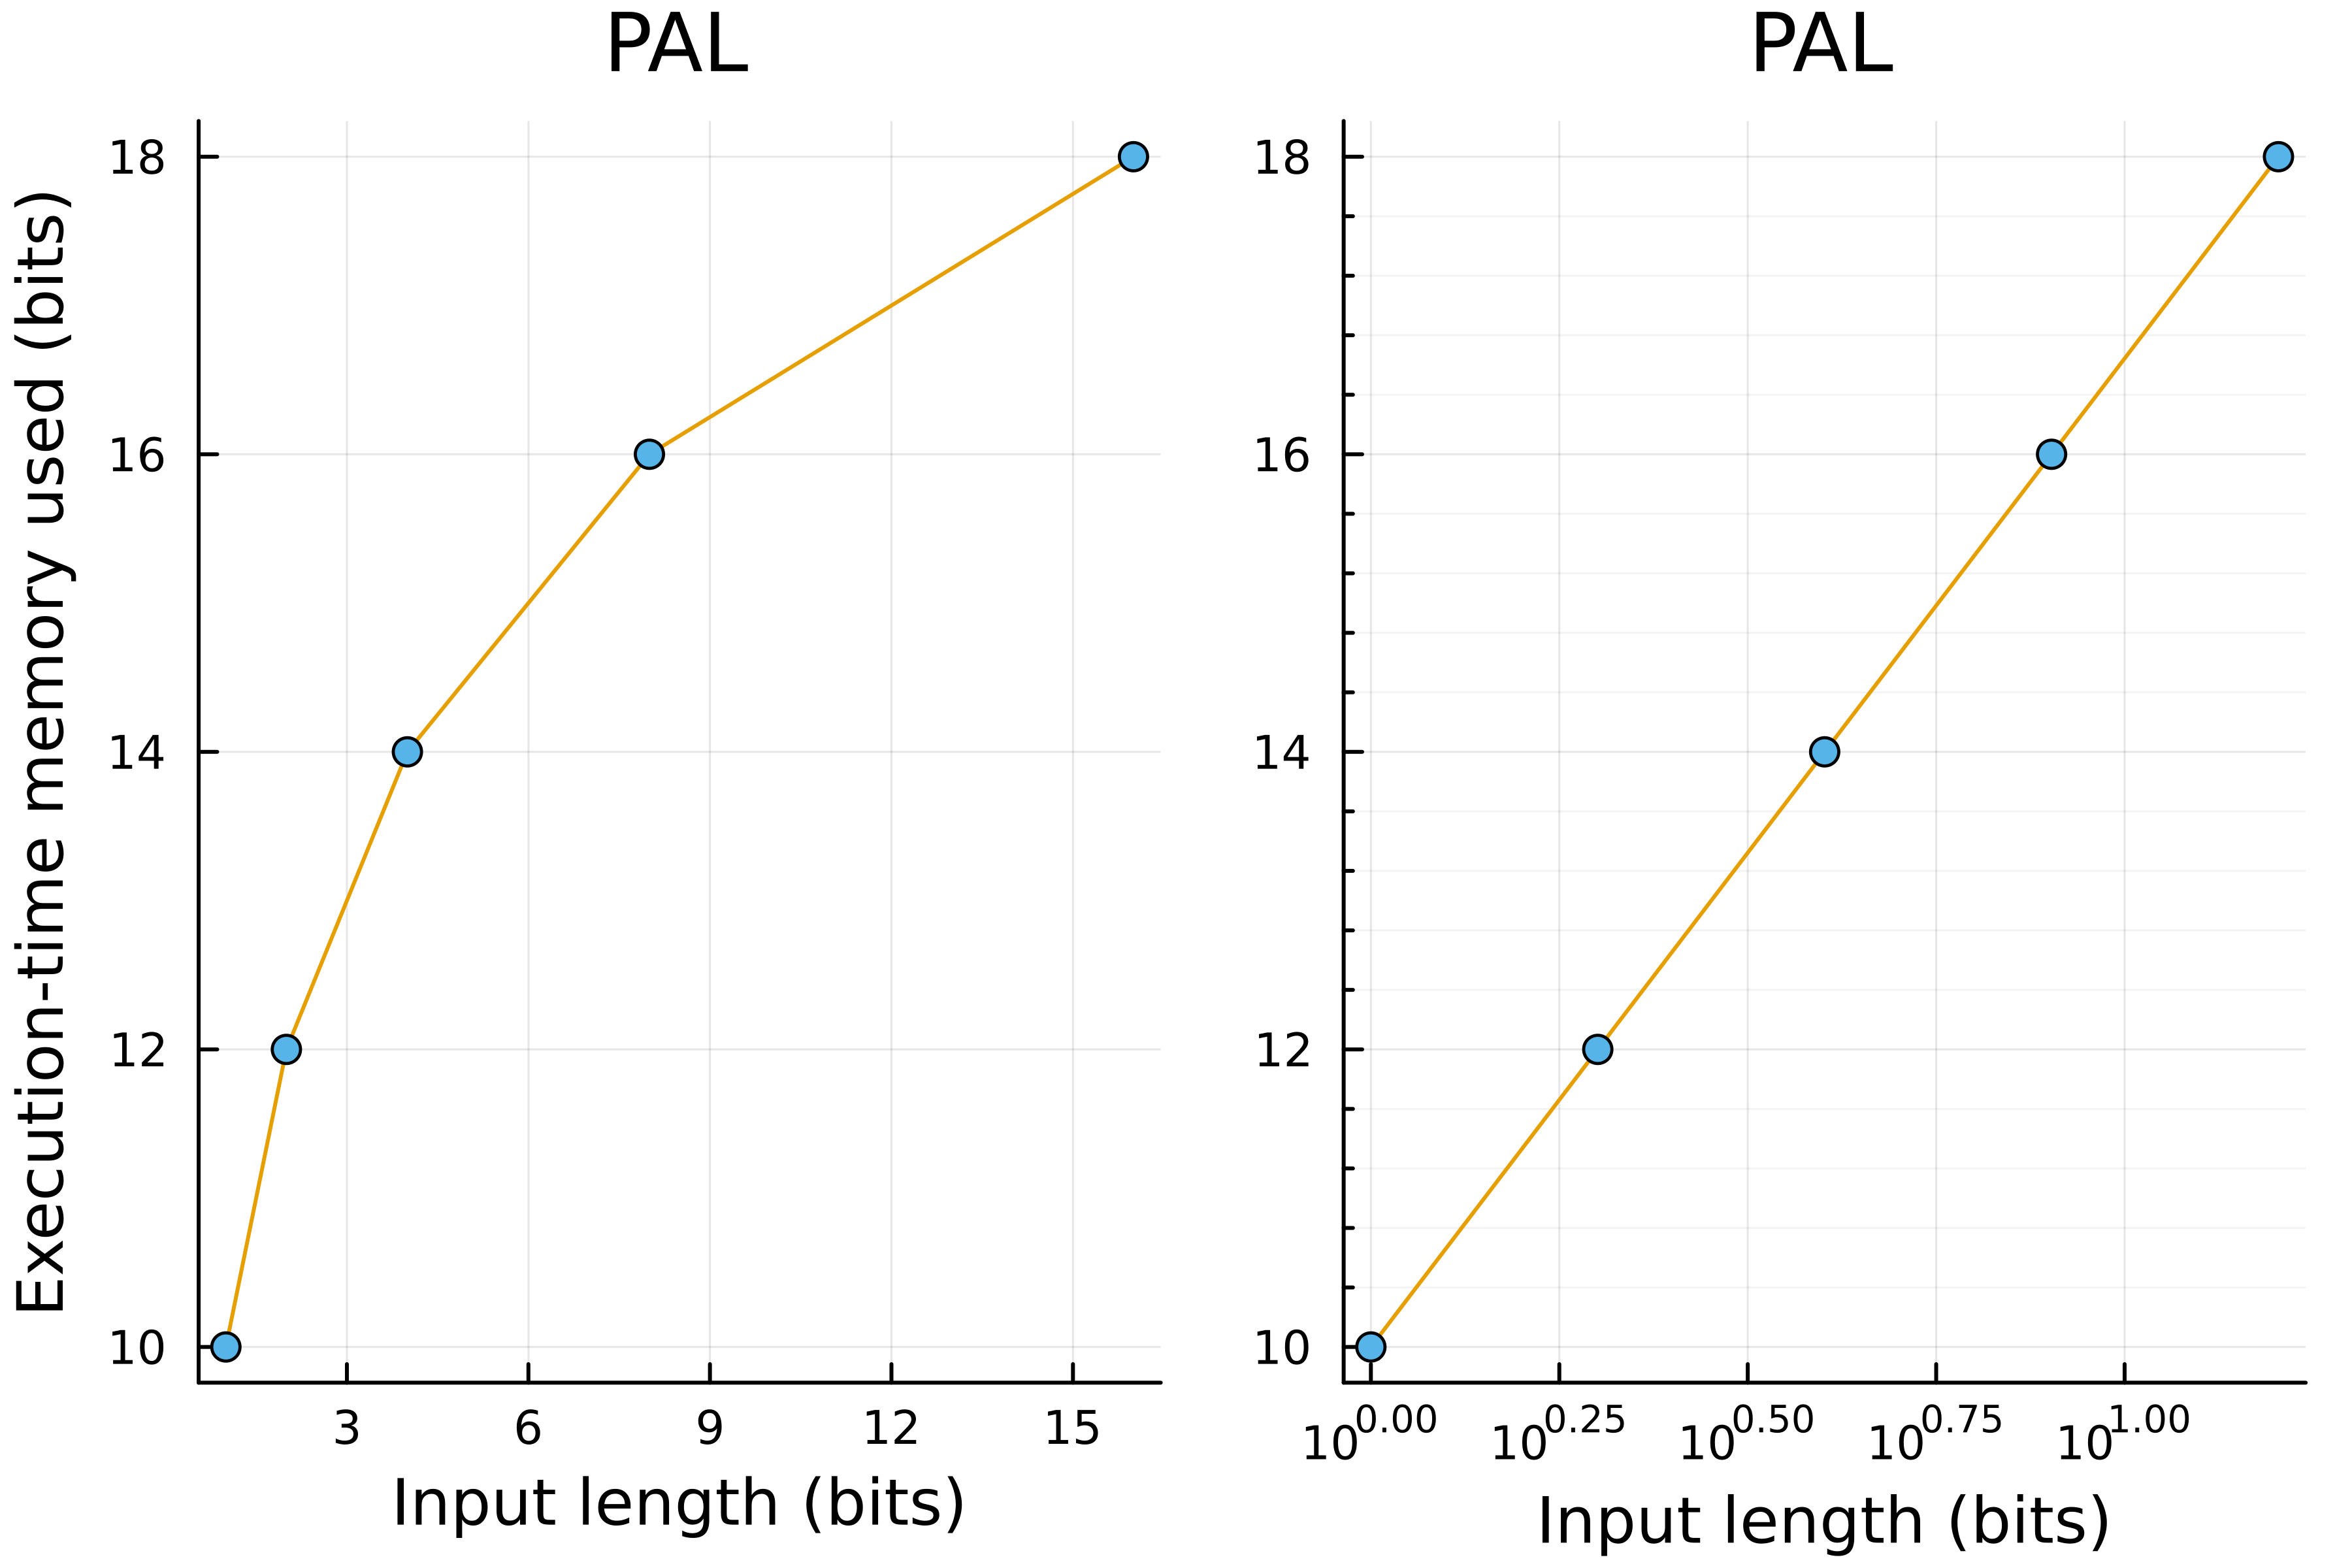
\includegraphics[width=\columnwidth]{PAL.png}
    \caption{Execution-time memory usage (bits) vs. input length (bits) for the LSPACE PAL algorithm given in Appendix \ref{app:pal}}
    \label{fig:pal}
\end{figure}

From these plots, it is clear that the PAL algorithm runs in logarithmic space relative to the input lengths.
This is the expected result.

I next tested Munin on an algorithm known to use linear space with respect to its input size.
This algorithm is a linear space ADD algorithm (LIN-ADD) that decides if \(x+y=z\).
The algorithm is shown in Appendix \ref{app:linAdd}.
It is known to be a linear space algorithm since it copies the inputs \(x\), \(y\), and \(y\).
Then, the algorithm adds \(x\) and \(y\) and compares it to \(z\).
Running LIN-ADD through Munin gives the following output:

\begin{lstlisting}
 COMPLEXITY ANALYSIS
----------------------------
 INPUT LENGTH | MEMORY USED 
--------------+-------------
 1            | 8      
--------------+-------------
 2            | 10      
--------------+-------------
 4            | 14      
--------------+-------------
 8            | 22      
--------------+-------------
 16           | 38      
\end{lstlisting}

This gives the following plots which validate that the algorithm runs in linear space, as expected:

\begin{figure}[H]
    \centering
    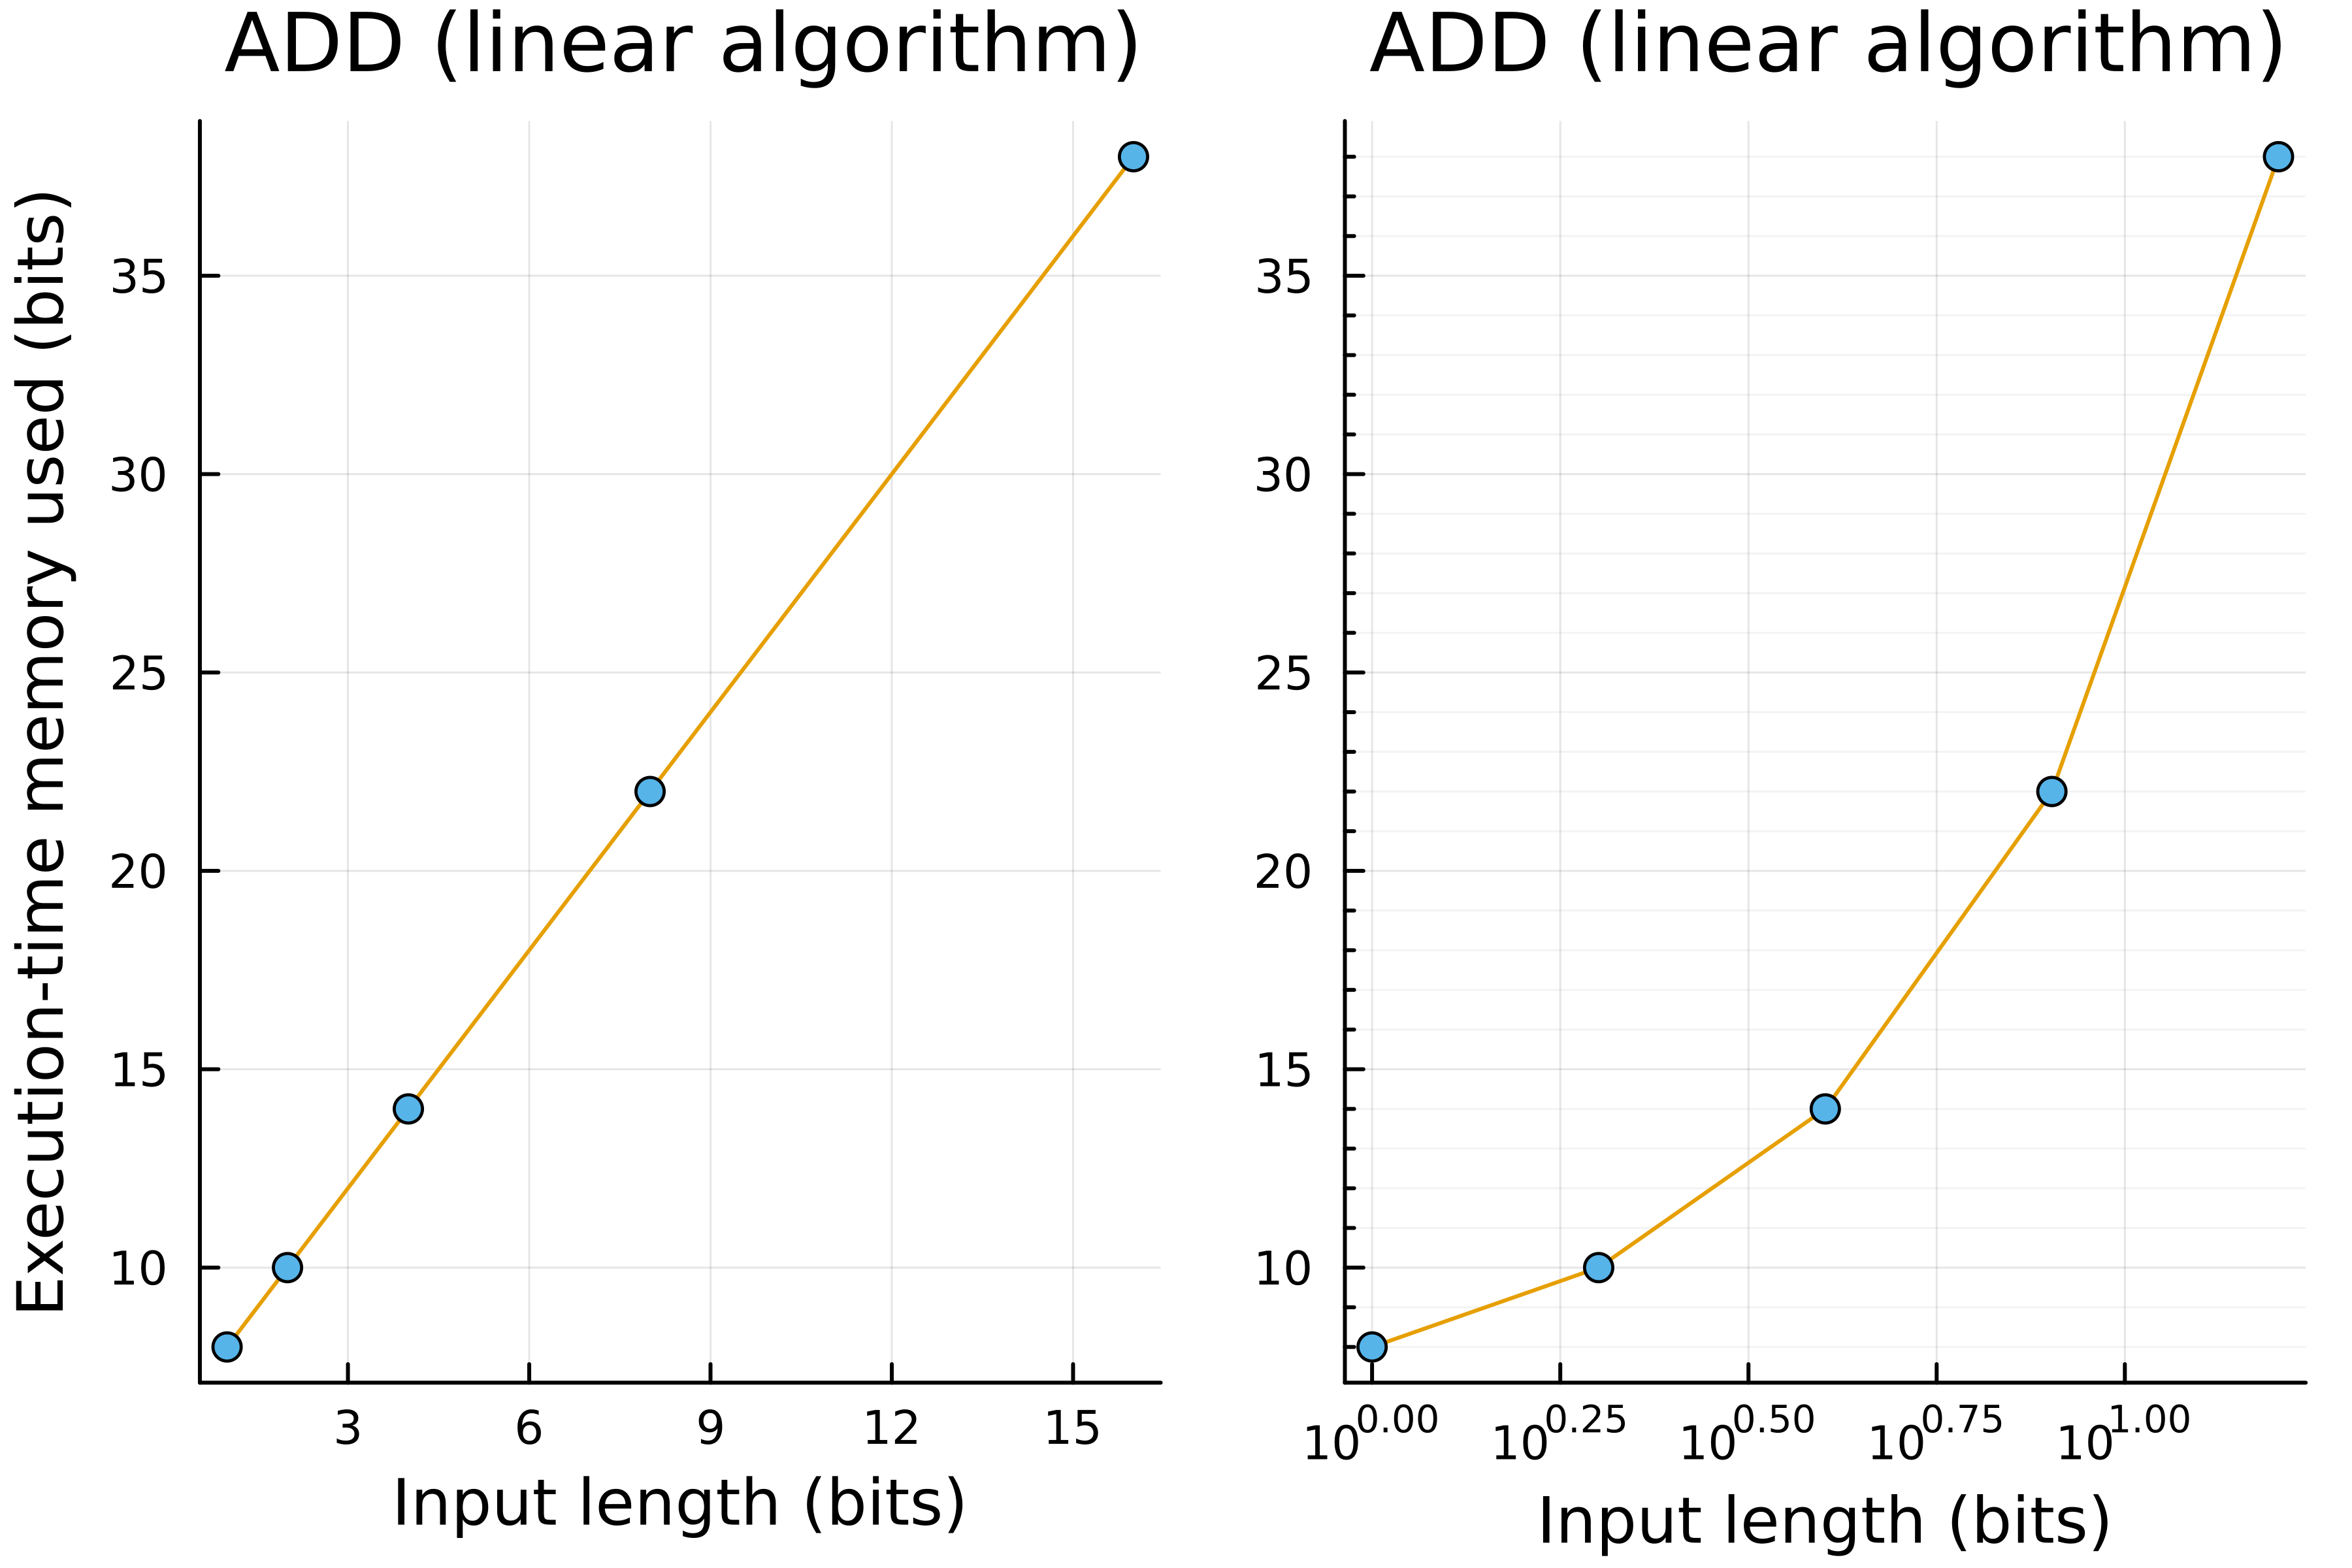
\includegraphics[width=\columnwidth]{ADD-(linear-algorithm).png}
    \caption{Execution-time memory usage (bits) vs. input length (bits) for the linear space ADD algorithm given in Appendix \ref{app:linAdd}}
    \label{fig:linAdd}
\end{figure}

An additional two algorithms are analyzed: PAL-ADD and ADD.
These are both algorithms that run in logarithmic space, proofs of this are written in \ref{app:proofs}.

The output and plot of running ADD through Munin is the following:

\begin{lstlisting}
 COMPLEXITY ANALYSIS
----------------------------
 INPUT LENGTH | MEMORY USED 
--------------+-------------
 1            | 10      
--------------+-------------
 2            | 12      
--------------+-------------
 4            | 14      
--------------+-------------
 8            | 16      
--------------+-------------
 16           | 18      
\end{lstlisting}

\begin{figure}[H]
    \centering
    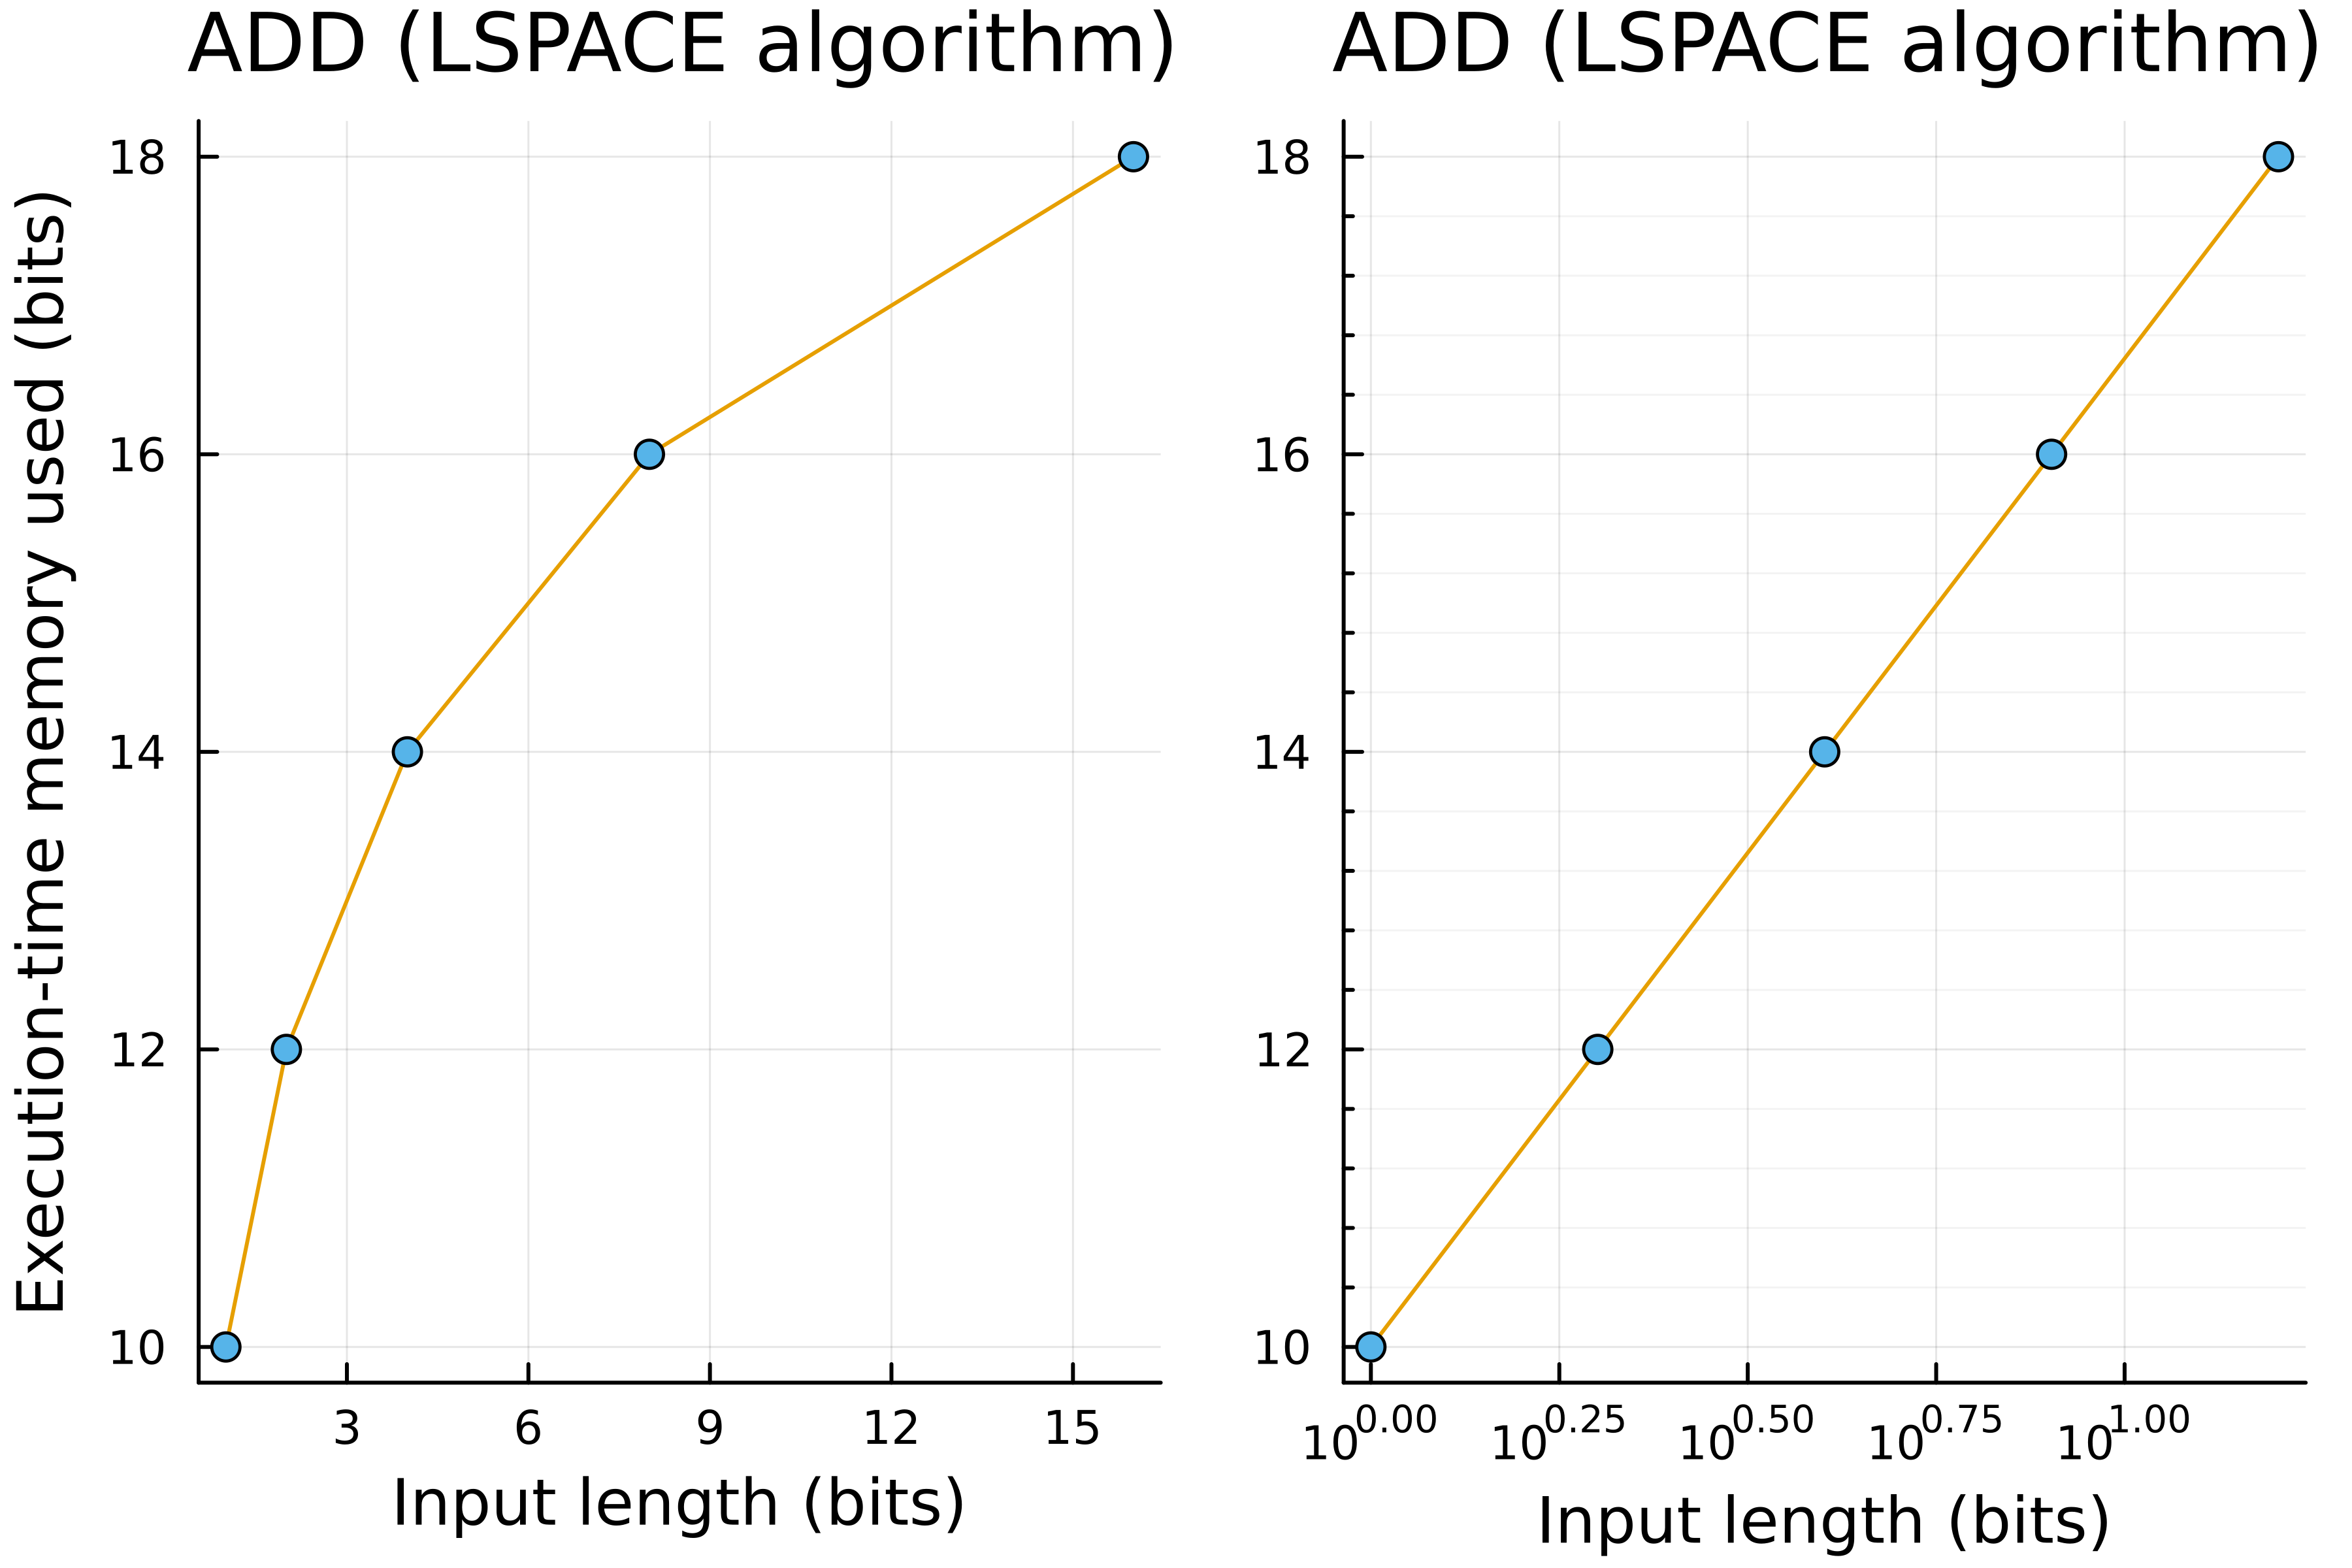
\includegraphics[width=\columnwidth]{ADD-(LSPACE-algorithm).png}
    \caption{Execution-time memory usage (bits) vs. input length (bits) for the LSPACE ADD algorithm given in Appendix \ref{app:lAdd}}
    \label{fig:lAdd}
\end{figure}

This demonstrates that ADD runs in logarithmic space or LSPACE.

The output and plot of running PAL-ADD through Munin is the following:

\begin{lstlisting}
 COMPLEXITY ANALYSIS
----------------------------
 INPUT LENGTH | MEMORY USED 
--------------+-------------
 1            | 20      
--------------+-------------
 2            | 25      
--------------+-------------
 4            | 30      
--------------+-------------
 8            | 35      
--------------+-------------
 16           | 40      
\end{lstlisting}

\begin{figure}[H]
    \centering
    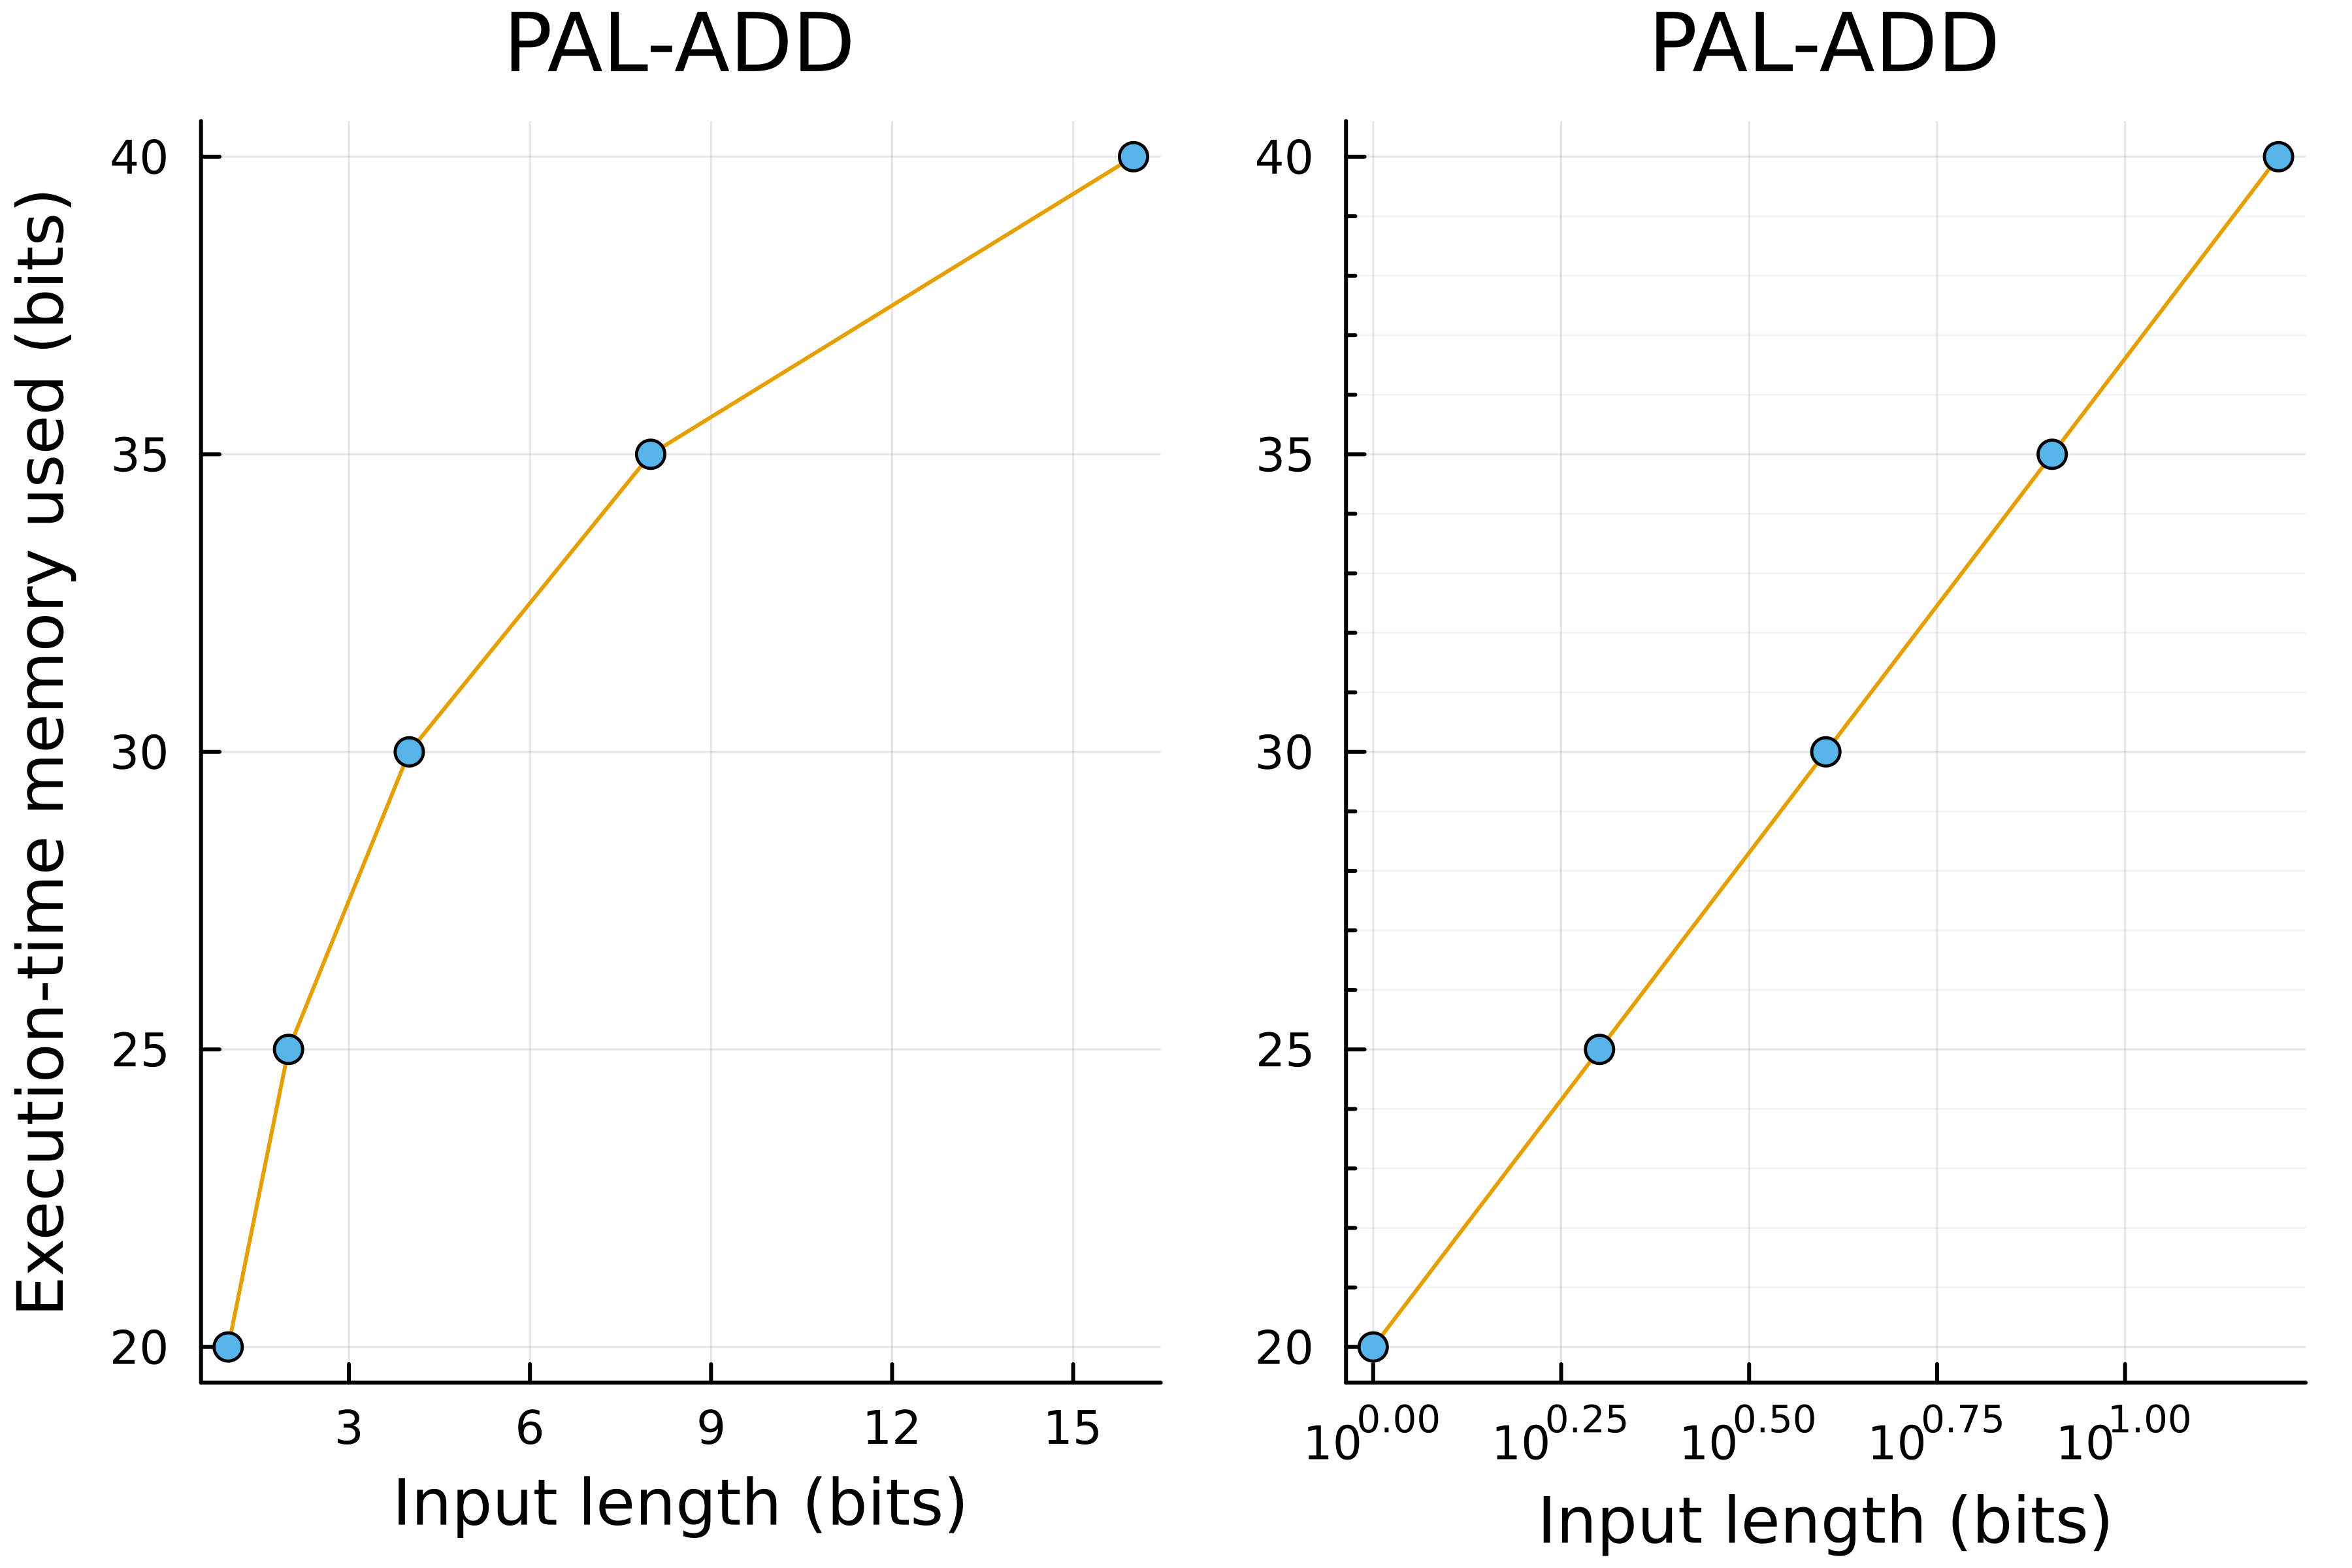
\includegraphics[width=\columnwidth]{PAL-ADD.png}
    \caption{Execution-time memory usage (bits) vs. input length (bits) for the LSPACE PAL-ADD algorithm given in Appendix \ref{app:palAdd}}
    \label{fig:palAdd}
\end{figure}

Likewise, this demonstrates that PAL-ADD runs in LSPACE.

\section{Discussion}

Here, I present Munin, a tool for measuring the execution-time memory usage of algorithms.
I show that Munin can be used to demonstrate and determine the theoretical space complexity of various programs.
I also demonstrate that LIN-ADD decides in linear space while PAL, ADD, and PAL-ADD decide in LSPACE.

The roadmap for future work on Munin first includes building a web-based application allowing users to write, run, and analyze Munin programs in the browser.
This will provide users a platform for easily exploring space complexity through writing and testing actual algorithms.
The next item on the roadmap is to expand the Munin assembly language to include `push` and `pop` operators and a function stack allowing users to write programs that include functions.
A final roadmap item is the creation of a scripting language, MuninScript, that compiles to the Munin assembly language.
This will allow users to more easily write Munin programs and study the space complexity of algorithms.

\newpage

\onecolumn

\appendix

\section{Munin example algorithms}

\subsection{LSPACE PAL algorithm}\label{app:pal}

\subsubsection{Pseudo-code}

\begin{lstlisting}[numbers=left]
    function pal(x)
        len = size_of(x)
        i = 0
        while i < len
            j = len - i - 1
            a = get_nth_bit_of(x, i)
            b = get_nth_bit_of(x, j)
            if a != b
                return false
            end
            i += 1
        end
        return true
    end
\end{lstlisting}

\subsubsection{Munin assembly code}

\lstinputlisting[numbers=left]{../examples/pal.asm}

\subsection{Linear-space ADD algorithm}\label{app:linAdd}

\subsubsection{Pseudo-code}

\begin{lstlisting}[numbers=left]
    function lin_add(x, y, z)
        a = x
        b = y
        c = z
        a += b
        if a != c
            return false
        end
        return true
    end
\end{lstlisting}

\subsubsection{Munin assembly code}

\lstinputlisting[numbers=left]{../examples/lin-add.asm}

\subsection{LSPACE ADD algorithm}\label{app:lAdd}

\subsubsection{Pseudo-code}

Note: it is assumed that the \lstinline|carry_flag| is set automatically when binary addition is performed and is set to \lstinline|false| at the start of each function.

\begin{lstlisting}[numbers=left]
    function add(x, y, z)
        len = size_of(z)
        i = size_of(x)
        if i > len
            return false
        end
        i = size_of(y)
        if i > len_z
            return false
        end
        i = 0
        while i < len
            x_bit = get_nth_bit_of(x, i)
            y_bit = get_nth_bit_of(y, i)
            if carry_flag
                x_bit = add_bits(x_bit, 1)
            end
            x_bit = add_bits(x_bit, y_bit)
            z_bit = get_nth_bit_of(z, i)
            if x_bit != z_bit
                return false
            end
            i += 1
        end
        return true
    end
\end{lstlisting}

\subsubsection{Munin assembly code}

\lstinputlisting[numbers=left]{../examples/add.asm}

\subsection{LSPACE PAL-ADD algorithm}\label{app:palAdd}

\subsubsection{Pseudo-code}

Note: it is assumed that the \lstinline|carry_flag| is set automatically when binary addition is performed and is set to \lstinline|false| at the start of each function.

\begin{lstlisting}[numbers=left]
    function pal_add(x, y)
        len = size_of(x)
        len_tmp = size_of(y)
        if len_tmp > len
            len = len_tmp
        end
        carry_on_last = carry_on_last_of_sum(x, y)
        i = 0
        while i < len
            i_bit = get_nth_bit_of_sum(x, y, i)
            j = len - i - 1 + carry_on_last
            j_bit = get_nth_bit_of_sum(x, y, j)
            if i_bit != j_bit
                return false
            end
            i += 1
        end
        return true
    end

    function get_nth_bit_of_sum(x, y, n)
        i = 0
        while i < n
            x_bit = get_nth_bit_of(x, i)
            y_bit = get_nth_bit_of(y, i)
            if carry_flag
                x_bit = add_bits(x_bit, 1)
            end
            x_bit = add_bits(x_bit, y_bit)
            i += 1
        end
        return x_bit
    end

    function carry_on_last_of_sum(x, y)
        len = size_of(x)
        len_tmp = size_of(y)
        if len_tmp > len
            len = len_tmp
        end
        i = 0
        while i < len
            x_bit = get_nth_bit_of(x, i)
            y_bit = get_nth_bit_of(y, i)
            if carry_flag
                x_bit = add_bits(x_bit, 1)
            end
            x_bit = add_bits(x_bit, y_bit)
            i += 1
        end
        if carry_flag
            return 1
        else
            return 0
        end
    end
\end{lstlisting}

\subsubsection{Munin assembly code}

\lstinputlisting[numbers=left]{../examples/pal-add.asm}

\newpage

\section{Proofs of space complexity}\label{app:proofs}

\subsection{ADD}

\begin{theorem} \label{thrm:add}
    \(\text{ADD} = \{\langle x, y, z \rangle : x + y = z\} \in L\)
\end{theorem}

\begin{proof}
    Let \(x, y, z\) be arbitrary binary integers.
    Here, it will be shown that if \(x + y = z\) can be decided in LOG-SPACE.

    Consider the ADD algorithm given in Appendix \ref{app:lAdd}.

    This algorithm determines if the sum of two binary integers \(x, y\) is a third binary integer \(z\).

    To show that it does so in LOG-SPACE, consider the variables used by \lstinline|add|.
    There are \(8\) such variables.
    \lstinline|x_bit|, \lstinline|y_bit|, \lstinline|z_bit|, and \lstinline|carry_flag| are all just a single bit each.
    \lstinline|len_x|, \lstinline|len_y|, \lstinline|len_z|, and \lstinline|i| can all hold values between \(0\) and \(n = max(n_x, n_y, n_z)\) where \(n_x, n_y, n_z\) are the sizes of \(x, y, z\) respectively in bits.
    Therefore, these four variables all require at most \(\log_2(n)\) bits.
    Thus, the total memory used by \lstinline|pal_add| is \(4\log_2(n) + 4\) bits meaning \lstinline|add| is a LOG-SPACE algorithm.

    Therefore, whether or not \(x + y = z\) can be decided in LOG-SPACE.
    Because \(x, y, z\) are arbitrary this is the case for any binary integers.
    
    Thus, \(\text{ADD} = \{\langle x, y, z \rangle : x + y = z\} \in L\).
\end{proof}

\subsection{PAL-ADD}

\begin{theorem}
    \(\text{PAL-ADD} = \{\langle x, y \rangle : x + y \text{ is a palindrome}\} \in L\)
\end{theorem}

\begin{proof}
    Let \(x, y\) be arbitrary binary integers.
    Here, it will be shown that if \(x + y\) is a palindrome can be decided in LOG-SPACE.

    Consider the PAL-ADD algorithm given in Appendix \ref{app:palAdd}.

    This algorithm determines if the sum of two binary integers is a palindrome.

    To show that it does so in LOG-SPACE, consider the variables used by \lstinline|pal_add|.
    There are \(7\) such variables.
    \lstinline|i_bit|, \lstinline|j_bit|, and \lstinline|carry_on_last| are all just a single bit each.
    \lstinline|len|, \lstinline|len_tmp|, \lstinline|i|, and \lstinline|j| can all hold values between \(0\) and \(n = max(n_x, n_y)\) where \(n_x, n_y\) are the sizes of \(x, y\) respectively in bits.
    Therefore, these four variables all require at most \(\log_2(n)\) bits.
    Thus, the total memory used by \lstinline|pal_add| is \(4\log_2(n) + 3\) bits meaning \lstinline|pal_add| is a LOG-SPACE algorithm.

    \lstinline|get_nth_bit_of_sum| and \lstinline|carry_on_last_sum| use the same program flow as \lstinline|add| from Theorem \ref{thrm:add} and use no more variables than \lstinline|add| does.
    Since Theorem \ref{thrm:add} shows that \lstinline|add| decides in LOG-SPACE, these do as well.
    Thus, all algorithms used in computing \lstinline|pal_add| use a logarithmic amount of space relative to the size of the input.

    Therefore, whether or not \(x + y\) is a palindrome can be decided in LOG-SPACE.
    Because \(x, y\) are arbitrary this is the case for any binary integers.
    
    Thus, \(\text{PAL-ADD} = \{\langle x, y \rangle : x + y \text{ is a palindrome}\} \in L\).
\end{proof}

\newpage

\section{Munin assembly reference}\label{app:asmRef}

\begin{tabular}[H]{| p{0.12\linewidth} | p{0.12\linewidth} | p{0.12\linewidth} | p{0.12\linewidth} | p{0.35\linewidth} |}
   
    \hline
    \multicolumn{5}{| c |}{Munin assembly reference}\\
    \hline
    \hline
    Operator & Operand 1 & Operand 2 & Operand 3 & Description\\
    \hline
    \multicolumn{5}{| c |}{Assignment operaions}\\
    \hline
    \lstinline|set| & \lstinline|D| & \lstinline|S| & & Sets variable D equal to the value of S\\
    \lstinline|stl| & \lstinline|D| & \lstinline|S| & & Sets variable D equal to the length of S\\
    \lstinline|stnb| & \lstinline|D| & \lstinline|S| & \lstinline|N| & Sets variable D equal to the Nth bit of S\\
    \hline
    \multicolumn{5}{| c |}{Integer arithmetic operaions}\\
    \hline
    \lstinline|iadd| & \lstinline|D| & \lstinline|S| & & Sets variable D equal to the value of D + S\\
    \lstinline|isub| & \lstinline|D| & \lstinline|S| & & Sets variable D equal to the value of D - S\\
    \hline
    \multicolumn{5}{| c |}{Binary arithmetic operaions}\\
    \hline
    \lstinline|badd| & \lstinline|D| & \lstinline|S| & & Sets one-bit variable D equal to the value of the binary sum of one-bit D and one-bit S; sets carry flag\\
    \lstinline|bsub| & \lstinline|D| & \lstinline|S| & & Sets one-bit variable D equal to the value of the binary subtraction of one-bit D and one-bit S; sets the underflow flag\\
    \lstinline|bsr| & \lstinline|D| & \lstinline|S| & & Sets variable D equal to the value of D << S\\
    \lstinline|bsl| & \lstinline|D| & \lstinline|S| & & Sets variable D equal to the value of D >> S\\
    \hline
    \multicolumn{5}{| c |}{Comparison operaions}\\
    \hline
    \lstinline|cmp| & \lstinline|A| & \lstinline|B| & & Sets the equal flag if A == B ; sets the greater flag if A > B\\
    \lstinline|clf| & & & & Clears all flags\\
    \hline
    \multicolumn{5}{| c |}{Program flow operaions}\\
    \hline
    \lstinline|jmp| & \lstinline|L| & & & Jumps to line L\\
    \lstinline|jon| & \lstinline|C| & & & Jumps over the next instruction if the condition C is true\\
    \lstinline|end| & & & & Ends the program\\
    
    \hline

\end{tabular}

\end{document}
